\documentclass[11pt, a4paper]{article} 
\usepackage{babel}
\usepackage{booktabs}
\usepackage{comment} 
\usepackage[utf8]{inputenc} % odpowiednie kodowanie znaków
\usepackage[T1, T2A]{fontenc} 
\usepackage{graphicx} %wstawianie obrazków
\usepackage{float} %ustawianie obraków/tabel
\usepackage{multirow}
\usepackage{amsmath, amsfonts,amsthm} 
\usepackage{amsthm} %do twierdzen itd
\usepackage{mathtools}
\usepackage{blindtext} 
\usepackage{geometry}
\usepackage{graphicx}
\usepackage{amssymb}
\usepackage{tikz-cd}
\usepackage{lscape}
\usepackage{hyperref}
\usepackage{XCharter}
\usepackage{dsfont}
\usepackage[labelfont=bf]{caption}
\usepackage{caption}
\usepackage{subcaption}
\usepackage{pbox}
\usepackage{tikz}
\usepackage{tikz-feynman}
\usepackage{svg}

\setlength{\parindent}{15pt} 

%%%%%%%%%%%%%%%%%%%%%%%%

\title{\vspace{-2cm}On the Landau pole in quantum electrodynamics and the possible quantum gravity corrections}
\author{{Wojciech Śmiałek}\\
\\
{\textit{Supervisor}} \\
{Jan Kwapisz phd.}}
\date{}

\begin{document}
\maketitle

\section*{Introduction}

\section{Standard model ...}
The Standard Model of particle physics is a unified description of all quantum fields observed in physics. 
It strives to predict all the phenomena observed at microscopic scales while maintaining theoretical
self-consistency and certain mathematical aesthetics. The predictive power of Standard Model, with its most
famous examples like precision tests of electron anomalous magnetic moment or the existence of Higgs' boson,
makes it ungrounded to postulate a fundamental physical theory that would not reduce to SM in the suitable limit, at least
as an effective field theory.
Standard Model, however, certainly is not a complete theory of physical reality. It does not include a description
of gravity and above the Planck scale $E_p \approx 10^{19} \ \text{GeV}$, due to quantum effects of gravity,
predictions of both the SM and Einstein's theory of gravity are not expected to apply.
One should then not be surprised, if at scales above $E_p$ Standard Model exhibits internal inconsistencies.
% Given the requirements of compatibility with SM and predictive power above the Planck scale, a criterion
% for any good theory of quantum gravity should be for it to resolve the problems that arise in SM due to absence of
% gravitational interaction.
One of the big issues of the SM is the quantum triviality problem for the electroweak $U(1)$ gauge coupling and
the scalar higgs boson quartic coupling.
In the pure electroweak theory, one loop $\beta$-function of the abelian gauge \cite{betaf scalar} \cite{betaf chiral lagrangian} is:% Ref higgs paper instead
\begin{equation}
    \beta_{g_Y}^{\text{SM}} = \beta_{g_Y}^{(3)} g_Y^3 = \frac{41}{6} \frac{g_Y^3}{16 \pi^2}
\end{equation}
This predicts a running of gauge coupling that would diverge at a momentum scale $\mu = \left(2 g_{Y\text{obs}}^2 \ \beta_{g_Y}^{(3)} \right)^{-1} $.
Conversely, taking any arbitrarily high value of the bare coupling, the only possible value of $g_{Y\text{obs}}$ should be 0, making
the theory trivial, i.e. non-interacting.
% In analogy to the QED fine structure constant, we define a dimensionless abelian gauge paramter as $\alpha_Y = g_Y^2 / 4 \pi$.
% It is related to the ordinary $\alpha_\text{QED}$ by a Weinberg angle and its value is known very precisely
% \begin{equation}
%     \alpha_Y = \frac{\alpha_\text{QED}}{\cos^2 \theta_W} = 0.0093905(30) % Two references to alpha and th_w, ogarnąć propagację niepewności
% \end{equation}
\begin{figure}[H]
    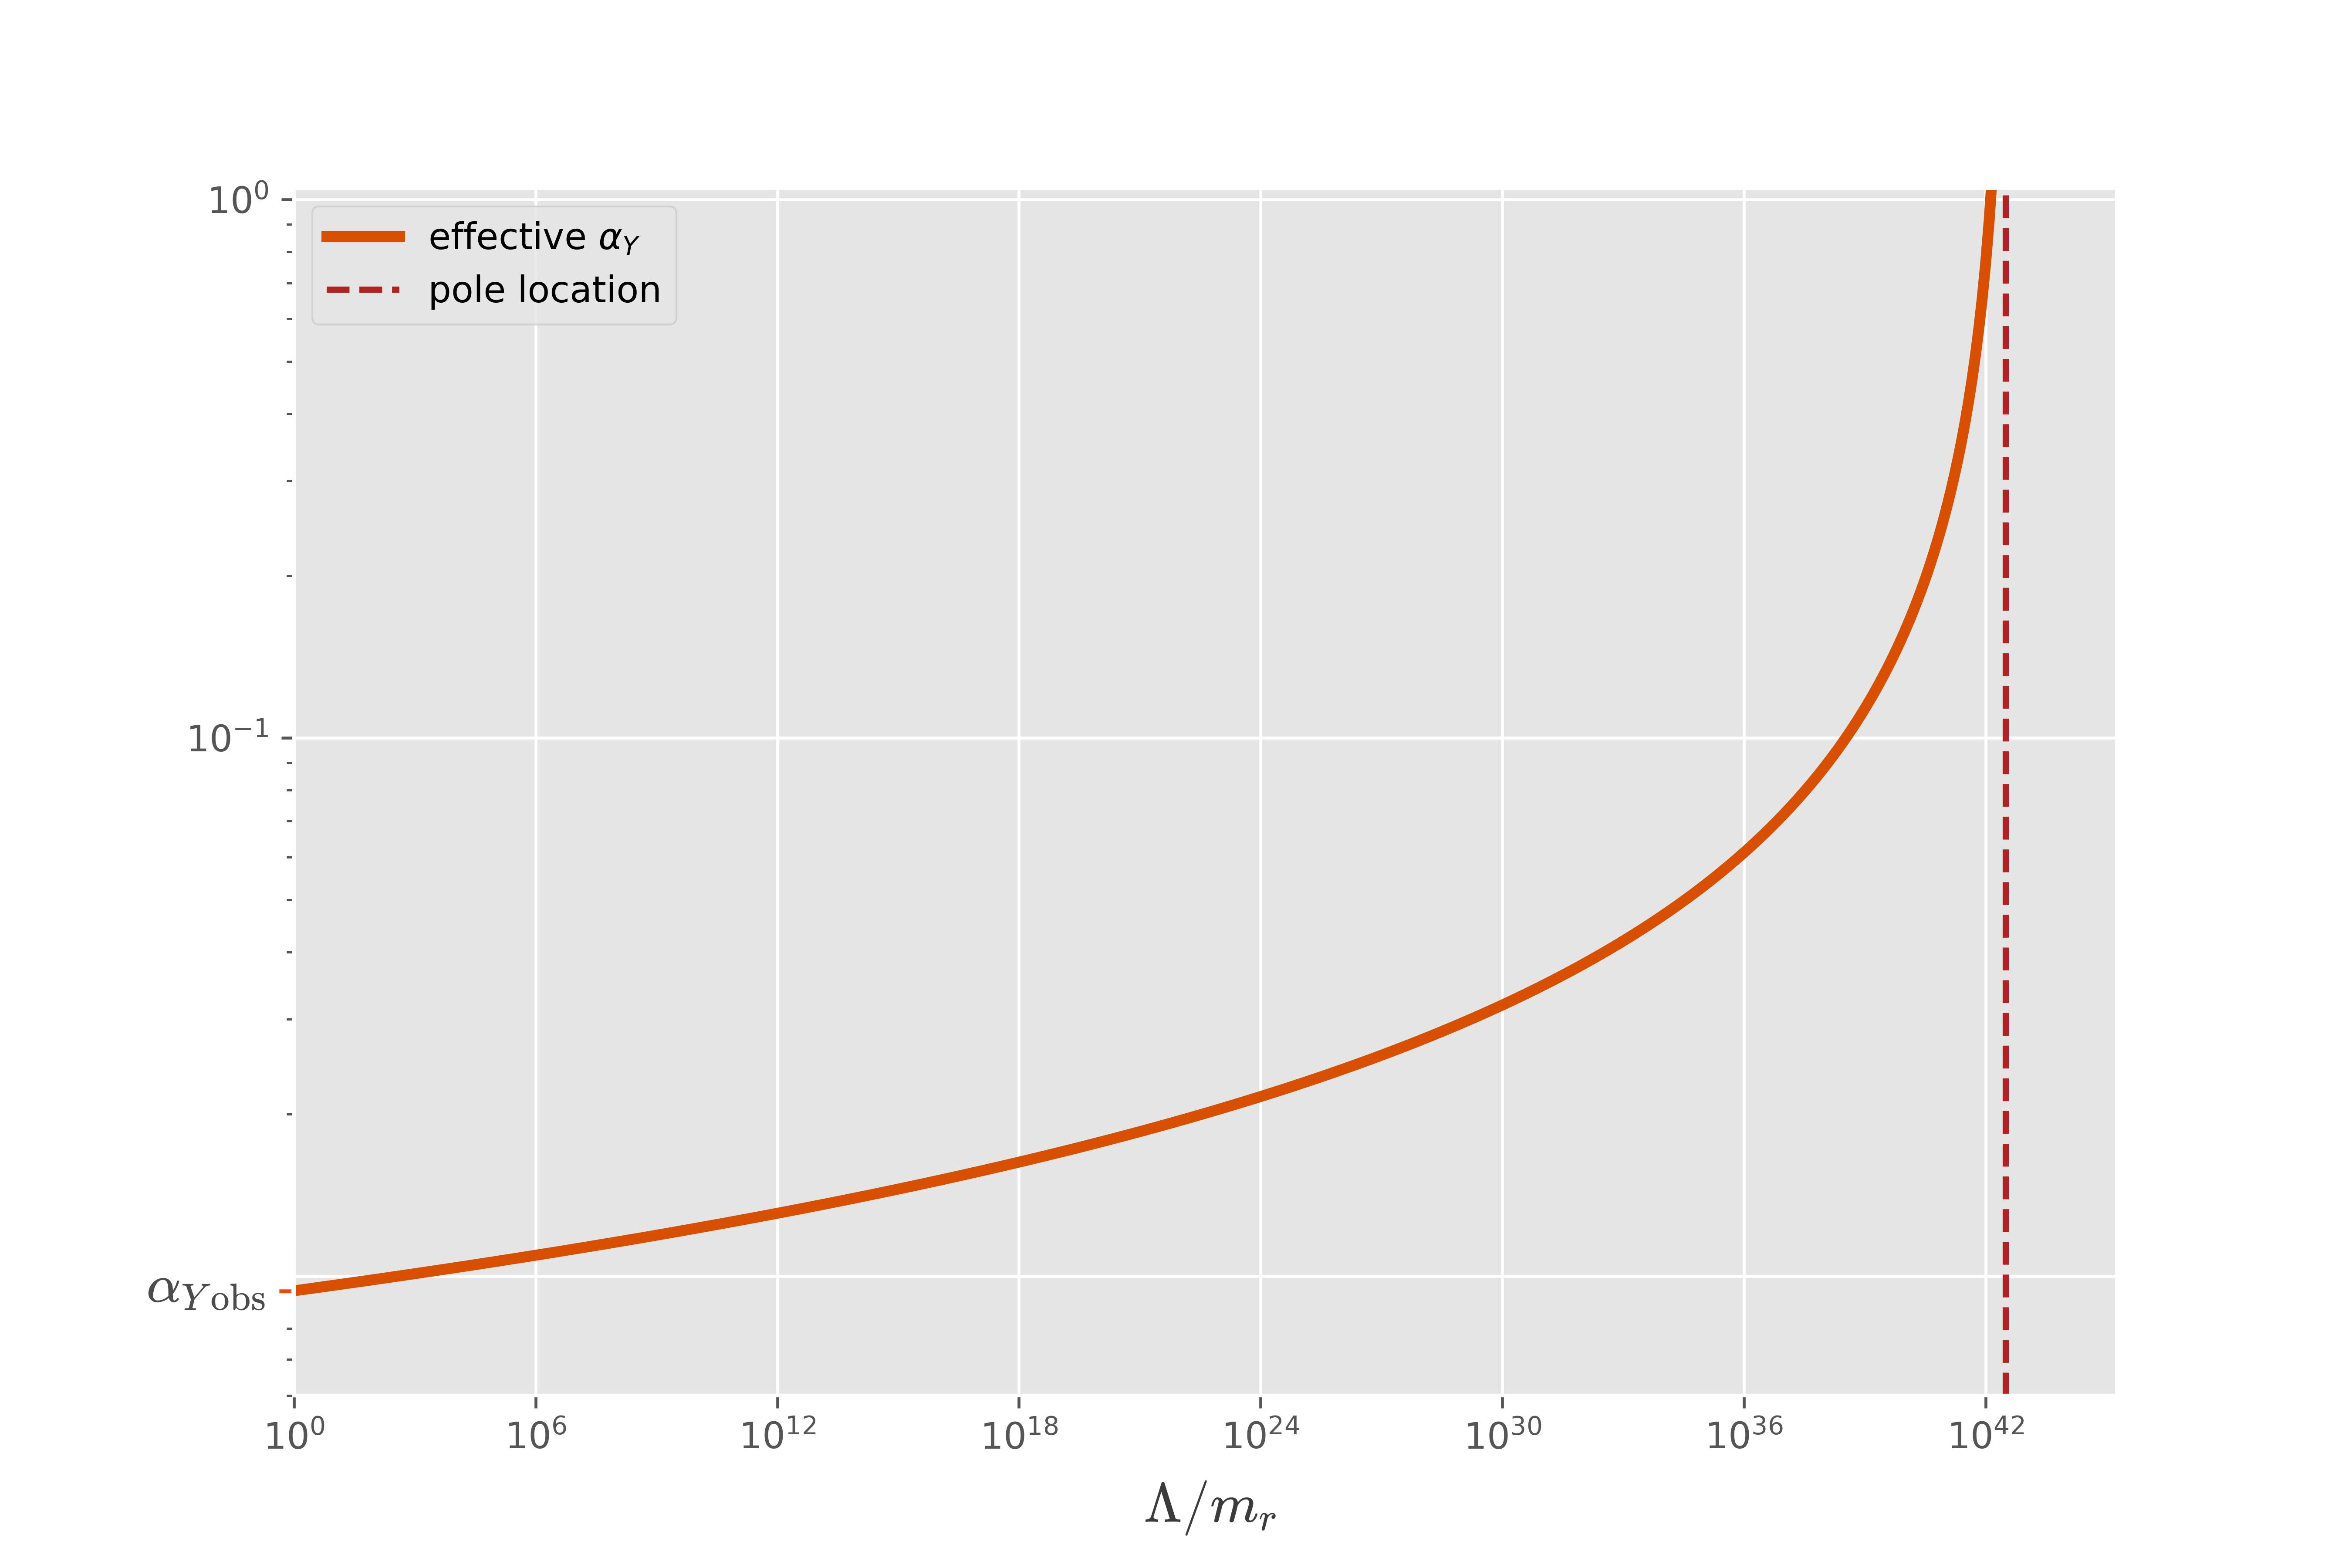
\includegraphics[width=1\textwidth]{./figures/plotr.jpg}
    \caption{Running of the abelian gauge parameter $\alpha_Y = \frac{g_Y^2}{4\pi}$. Observed value $\alpha_{Y\text{obs}}$ is taken from [refs]. 
    Landau Pole marked at $\mu \approx 10^{42.5}$}
    \label{boxes}
\end{figure} 
Taking an electron mass as a reference scale, the location of abelian coupling landau pole will be of order $\Lambda \sim 10^{48} \ \text{eV}$, well above the Planck scale.
Similarly, quartic self-interaction of higgs field theoretically may exhibit a pole at a finite momentum scale.
Existence of both poles remains an open question, but a theory containing any such singularity cannot be fundamental.
One solution to this problem could be a grand unified theory (GUT), which proposes a larger symmetry group, spontaneously broken
to the known $SU(3)\times SU(2) \times U(1)$ of standard model at around the scale where running values of electroweak and strong couplings
coincide. This scale is predicted to be below planck energy [ref]. Above it, the theory could introduce
a running of unified coupling that does not exhibit a triviality issue.
The existence of grand unification, however has not been yet confirmed in any way, while the experimental bounds on the proton lifetime
heavily constraints or even rules out many of the GUTs[ref]. This constrasts sharply with the other potential completion of the SM,
which is quantum gravity. Although no quantum theory of gravity has been widely accepted, the existence of gravity and
the quantum nature of physical reality most certainly are. Should quantum gravitational solution to the triviality issues of the SM exist,
it could provide an argument of consistency between the particular theory of quantum gravity and the SM, as well as eliminate one of the arguments for the need of GUT.

% For a (canonical) quantum field theory of gravity, the use of perturbative methods results in the loss of predictive power, if the theory is
% postulated to be fundamental. Due to the breakdown of perturbative methods , 

\textcolor{red}{(discussion of results outside asymptotic safety paradigm. Wilczek, pro and contra, etc.)} 

% (I tutaj napisać jak AS to rozwiązało i przewidziało masę higgsa więc dobry trop i wogle)
% Wspomnieć że jeżeli biegun landaua zostanie, to nasz model musi być no najwyżej teorią efektywną
% I dopisać że do przewidzenia masy higgsa potrzeba żeby wkład od grawitacji do U(1) był ujemny, co my tutaj pokazujemy

% For the abelian gauge coupling $g$ with vanishing
% canonical dimension, the Ward-Takahashi identities imply a relation between the $\beta$-function of the coupling and the anomalous
% dimension $\eta_A$ of the gauge field. In the pure electroweak theory 
% Landau Pole
% Landau Pole for abelian hypercharge - figure
% + AS resolution of higgs triviality

% Ogólnie problemy SM
% Grand unification vs brak rozpadu protonu i prospects
% Alternatywa dla potrzeby gut - częścią tego istnienie fixed point of abelian coupling przy dodaniu grawitacji

\section{Asymptotic safety ...}

\subsection{The Functional Renormalization Group Equation}

% \subsubsection*{\centering Effective action}

% In the traditional Wilsonian approach to renormalization, a single step of renormalization procedure consists of
% a functional integration of high-momentum fluctuations, followed by a rescaling of physical lengths and momenta, and
% renormalization of fields. All of this leaves the non-perturbed theory unchanged, affecting only the couplings.
% Before the rescaling and renormalization operations [we are dealing with] the so-called Wilsonian effective action ($S_{\text{eff}}$).
% It describes the behaviour of fields for the processes below certain energy scale $b\Lambda$, lower than the original cutoff $\Lambda$.
% $S_{\text{eff}}$ generally contains all operators with higer dimensions in fields and derivatives.
% These corrections (...) but they allow us to neglect field modes larger than $\mu = b\Lambda$ and deal only with non-divergent diagrams.
% The argument of $S_{\text{eff}}$ is still a quantum field, in the sense that the functional integral is performed over it. %It also,
% in some sense, loses information about the high-energy physics.

The central object of the functional renormalization group is the effective average action.
% The object, that we will call an effective action $\Gamma$ is different and should not be confused with $S_{\text{eff}}$.
To introduce it, let us start from the scalar field theory. The definition for other theories come as a straight-forward generalization.
Its euclidean partition function and the generating functional of connected Green's functions reads
\begin{gather}
    Z[j] = \int \mathcal{D}\phi \ e^{-S[\phi] + \int dx j \phi} \\
% \end{equation}
% % The generating functional of connected Green's functions is defined as
% \begin{equation}
    W[j] = \log{Z[j]}
\end{gather}
The effective action functional is then defined using the Legendre transform of $W[j]$.
\begin{equation}
    \Gamma[\phi_c] = W[j_\phi] - \int d^4 x j_\phi(x) \phi(x)
\end{equation}
The two fields $\phi_c$ and $j_\phi$ are inverses of each other, defined as the solution to
\begin{equation}
    \phi_c(x) = \langle \hat\phi (x) \rangle_j = \frac{\delta W[j]}{\delta j(x)}
\end{equation}
The argument of the effective action is a classical field and there is no functional integral to be performed over it.
Rather, in $\Gamma$ all of the fluctuations are integrated out, but only one-particle irreducible diagrams
are included. $\Gamma$ acts as a generating functional of 1PI Green's functions. Extremizing effective, rather than
the clasical action, yields the equations of motion for vacuum expectation values of the quantum fields.

In its bare form, effective action is ill-defined, as was expected. One option is to introduce a UV cutoff $\Lambda$
and study the rg flow through divergences proportional to $\Lambda$. The modification we will employ, however, involves
an IR cutoff inserted through adding a regulator term $\Delta S_k[\phi]$ to the bare action $S[\phi]$ in the definition of partition function
and subtracted from the final form of effective action. Explicitly, this new object, called the effective average action (EAA) is defined as
\begin{gather}
    W_k[j] = \log{\int \mathcal{D}\phi \ e^{-S[\phi] - \Delta S_k[\phi] + \int dx j \phi}}\\
    \Gamma_k[\phi_c] = W_k[j_\phi] - \int d^4 x j_\phi(x) \phi(x) - \Delta S_k[\phi]
\end{gather}
Motivation for this definition of EAA will become clear when we study the functional renormalization group

% \subsubsection*{\centering Infrared regulator and the scheme dependence}
\textcolor{red}{(Infrared regulator and the scheme dependence)}
% \subsubsection*{\centering Beta functional and the functional renormalization group}

The $\Gamma_k$ is IR-regulated, but the UV divergences still cause it to be ill-defined. 
However, in studying the scale dependence of couplings we will not use full EAA, 
but its derivative with respect to $t = \log{k}$.
We assume the theory space in which $\Gamma_k$ takes the form
\begin{equation}
    \Gamma_k = \sum_i g_i(k) \ \mathcal{O}_i [\phi]
    \label{gamma_decomp}
\end{equation}
Where $\mathcal{O}_i (\phi)$ are integrals of monomials of fields or positive powers of field derivatives 
and $g_i(k)$ are scale-dependent couplings.
The coefficients in the derivative $\partial_t \Gamma_k$ are therefore simply the beta functions of corresponding operators
\begin{equation}
    \frac{d \Gamma_k}{dt} = \sum_i \frac{d g_i}{dt} \ \mathcal{O}_i [\phi] = \beta_i(g,k) \ \mathcal{O}_i [\phi]
\end{equation}
The beta functions may depend on all the couplings, as well as the renormalization scale $k$.
They can be extracted from $\frac{d \Gamma_k}{dt}$ via a suitable projection operator. 
The $\frac{d \Gamma_k}{dt}$ is called the beta functional and it is finite and well-defined [refs].
This is because the beta functional can be viewed as a difference between effective actions with infinitesimally
different cutoffs, where the UV divergences in the difference cancel and what remains is the finite rest
dependent on the degrees of freedom with momenta close to the renormalization scale.
At the one loop level, the derivative of effective average action can be expressed as
\begin{equation}
    \frac{d \Gamma_k^{(1)}}{dt} = \frac{1}{2} \operatorname{Tr} \left[ \left(\frac{\delta^2 S}{\delta \phi \delta \phi} + R_k\right)^{-1} \cdot \frac{d R_k}{dt} \right]
\end{equation}
Which follows from the known expression for the one-loop effective action [ref].
One may guess, that the "renormalization group improvement" of this equation - the replacement of ordinary action by
 EAA, will lead to a more accurate description of physics:
\begin{equation}
    \frac{d \Gamma_k}{dt} = \frac{1}{2} \operatorname{Tr} \left[ \left(\frac{\delta^2 \Gamma_k}{\delta \phi \delta \phi} + R_k\right)^{-1} \cdot \frac{d R_k}{dt} \right]
    \label{FRGE}
\end{equation}
As it turns out, this equation is proved to be exact and does not rely on any perturbative expansion [refs].
It is called the functional renormalization group equation (FRGE) or the Wetterich equation.
It is a simple, first order differential equation that governs the renormalization group flow of $\Gamma_k$ functional.

% Let us calculate the derivatives of $W_k$ and $\Delta S_k$ with respect to $t$
% \begin{gather}
%     \frac{d W_k}{dt} = \frac{d}{dt}\log{Z_k} = - \frac{1}{Z_k} \int \mathcal{D}\phi \ e^{-S[\phi] - \Delta S_k[\phi] + \int dx j \phi}  \cdot \frac{d \Delta S_k}{dt} \\
%     \frac{d \Delta S_k}{dt} = \frac{1}{2} \int d^4 x \ \phi \ \frac{d R_k}{dt} \ \phi
% \end{gather}
% This lets us write
% \begin{equation}
%     \frac{d \Gamma_k}{dt} = \frac{d \langle \Delta S_k \rangle}{dt} - \frac{d \Delta S_k }{dt} = \frac{1}{2} \operatorname{Tr} \left[ (\langle\phi\phi\rangle - \langle\phi\rangle^2) \cdot \frac{d R_k}{dt} \right]
% \end{equation}
% Where $\operatorname{Tr}$ denotes ... and the $\langle\cdots\rangle$ - ...
% The expression $(\langle\phi\phi\rangle - \langle\phi\rangle^2)$ can be shown to be equal to $\frac{\delta^2 W_k}{\delta j \delta j}$ [cite]
% From there, if we would express $\frac{\delta^2 W_k}{\delta j \delta j}$ in terms of $\Gamma_k$, we could
% write an exact, first order differential equation for the effective average action.
% In fact, the relationship between (them) is very simple. Recall, that $\Gamma_k + \Delta S_k$ is a Legendre transform of $W_k$. For any
% two functions $f$ and $g$, one being the Legendre transform of the other, we have $f'' = (g'')^{-1}$. This remains true for the functional derivation.
% Using this information and immediatly performing field derivative over $\Delta S_k$, we can write the equation for $\Gamma_k$:
% \begin{equation}
%     \frac{d \Gamma_k}{dt} = \frac{1}{2} \operatorname{Tr} \left[ \left(\frac{\delta^2 \Gamma_k}{\delta \phi \delta \phi} + R_k\right)^{-1} \cdot \frac{d R_k}{dt} \right]
%     \label{FRGE}
% \end{equation}
% This is the functional renormalization group equation (FRGE) or the Wetterich equation. (...)
In its original form, FRGE is not well suited for performing specific calculations. One very intuitive method, which
we will use, is called the $\mathcal{PF}$-expansion. 
% that allows us to use the Feynman diagrams for calculating the RHS of equation (\ref{FRGE}) up to the desired order in couplings. 
The term inside the trace including Second derivative of EAA
will in general be, for spinor or tensor fields, a functional hessian matrix. We can decompose this term into a
regulated inverse propagator matrix $\mathcal{P}$ and a rest, which will include the derivatives of terms non quadratic in fields.
\begin{equation}
    \frac{\delta^2 \Gamma_k}{\delta \phi \delta \phi} + R_k = \mathcal{P} + \mathcal{F}
    \label{pf1}
\end{equation}
First, let us notice that the entire expression inside trace can be expressed as a $\log{(\mathcal{P}+\mathcal{F})}$, upon which acts
a $t$-derivative sensitive only on the $t$ dependence in $R_k$. Explicitly, we can write:
\begin{equation}
    \left(\mathcal{P} + \mathcal{F}\right)^{-1} \cdot \partial_t R_k = \left(\mathcal{P} + \mathcal{F}\right)^{-1} \cdot \widetilde{\partial_t} \left(\mathcal{P}+\mathcal{F}\right) = \widetilde{\partial_t} \log{\left(\mathcal{P}+\mathcal{F}\right)}; \quad \widetilde{\partial_t} = \int \partial_t R_k \frac{\delta}{\delta R_k}
\end{equation}
Now, we can recall the series expansion of $\log{(1+x)}$ around $x=0$ and after some simple manipulations, obtain an expansion of functional trace in (\ref{FRGE}) in
the number of $\mathcal{F}$-terms
\begin{gather}
    \frac{d \Gamma_k}{dt} = \frac{1}{2} \operatorname{Tr} \left[ \widetilde{\partial_t} \log{\left(\mathcal{P}+\mathcal{F}\right)} \right] = \frac{1}{2} \operatorname{Tr} \left[ \widetilde{\partial_t} \left(\log{\mathcal{P}} + \log{(1+\mathcal{P}^{-1}\mathcal{F})}\right) \right] \\ =  \frac{1}{2} \operatorname{Tr} \left[ \widetilde{\partial_t} \log{\mathcal{P}} \right] + \frac{1}{2} \sum_{n=1}^{\infty} \frac{(-1)^{n-1}}{n} \operatorname{Tr}\left[\widetilde{\partial_t}\left(\mathcal{P}^{-1}\mathcal{F}\right)^n\right]
    \label{pf}
\end{gather}
Using this expression, we can reduce the problem of finding $\partial_t \Gamma_k$ to computing a set of feynman diagrams.
% For the computation of 
% Even though this method appears to again rely on a small expansion parameter, 

% As the Landau Pole of abelian coupling is situated well above the Planck scale, one can conjecture that
% its existence is due to the abence of quantum gravitational effects in the theory.
% Even without postulating a UV-complete gravitational theory, it is beneficial to investigate
% the impact of graviton on the running of abelian coupling [Wilczek ... czy coś]


% QED is a perturbatively renormalizable theory, i.e. it allows to calculate probability amplitudes for physical processes
% up to an arbitrary order in couplings.
%% One loop beta function of qed
%% Discussion of landau pole
%% General form in the presence of quantum gravity
% Wilczek paper
%% Qualitative difference

\textcolor{red}{(discussion of results in asymptotic safety, results obtained in this work and the general conclusion)} 

\section{Obtained results ...}

\subsection{Calculations}

A great advantage of functional renormalization group is that, if all terms
allowed by the symmetries are included in the effective action, one obtains a set of first order
differential equations containing full information about the RG flow in the theory, without referring to the perturbative methods.
For typical theories, that means an infinite set of coupled differential equations.
What allows calculations to be feasible, is considering only a manageable subset of terms in the effective action, the so-called truncation method.
For a good choice of truncation, adding subsequent terms beyond this subset will contribute to beta functions in a negligible way
and the results will be a good approximation of the actual behaviour of the theory.

In the present calculations, the following truncation of effective action is assumed:
\begin{equation}
    \Gamma = \int d^4 x \left( \mathcal{L}_{EH} + \mathcal{L}_A + \mathcal{L}_{GGF} + \mathcal{L}_{AGF} \right) \\
\end{equation}
The gravitational sector consists of the Einstein - Hilbert action with a cosmological constant $\Lambda$ and a gravitational gauge fixing term
\begin{gather}
    \mathcal{L}_{EH} = \sqrt{\mathbf{g}} \ \frac{k^2}{\kappa} \left( k^2 \Lambda - R(\partial)\right) \\
    \mathcal{L}_{GGF} = \sqrt{\mathbf{g}} \ Z_h \frac{1}{32 \pi \alpha_h} \left(\partial_\mu h^{\mu\nu} - \frac{1+\beta_h}{4} \partial^\nu h^\rho_{\; \rho} \right)^2\\
\end{gather}
Whereas the gauge sector contains a kinetic term of the photon
% , effective four-photon interaction 
and a gravitational gauge fixing term
\begin{gather}
    \mathcal{L}_A =  \sqrt{\mathbf{g}} \left( Z_A \frac{1}{4} F^{\mu\nu} F_{\mu\nu} \right)\\% + w_2 (F^{\mu\nu} F_{\mu\nu})^2 \right)\\
    \mathcal{L}_{AGF} = \sqrt{\mathbf{g}} \ Z_A \frac{1}{2 \alpha_A} \left( \partial_\mu A^\mu \ \partial_\nu A^\nu \right) \\
\end{gather}

%% Fourier transforms of lagrangian etc

The effective action can be represented as a functional dependending only on the fourier transform of gauge and graviton fields.
\begin{gather}
    \Gamma\left[ A^\mu, h^{\mu\nu}, \partial_\mu A^\mu, \partial_\mu \partial_\nu h^{\mu\nu}, \cdots\right] = \Gamma[ \tilde{A}^\mu, \tilde{h}^{\mu\nu}] \\
    \tilde{\phi}(p) = \mathfrak{F}[\phi] = \int d^4 x e^{-i p_\mu x^\mu} \phi(x)
\end{gather}
When we express the fields in effective lagrangian by $\phi(x) = \mathfrak{F}^{-1}[\tilde{\phi}(p)]$,
any spacetime derivative $\partial_\mu \phi^\mu(x)$ can be replaced by $i p_\mu \tilde{\phi}^\mu(p)$.
By further rearrangements and performing spacetime integral, we can arrive at the momentum-space lagrangian,
depending only on $\tilde{\phi}$
\begin{align}
    & \int d^4 x \prod_i \partial_{\mu_i} \phi^{\mu_i}(x) \prod_j \phi^{\nu_j} = \\
    & = \int d^4 x \int \left( \prod_i d^4 p_i i p_{i_{\mu_{i}}} \tilde{\phi}^{\mu_i}(p_i)\right)\left( \prod_j d^4 p_j \tilde{\phi}^{\nu_j}(p_j)\right) e^{i x \left(\sum_i p_i + \sum_j p_j \right)} \\
    & = \int \left( \prod_i d^4 p_i i p_{i_{\mu_{i}}} \tilde{\phi}^{\mu_i}(p_i)\right)\left( \prod_j d^4 p_j \tilde{\phi}^{\nu_j}(p_j)\right) \delta\left( \sum_i p_i + \sum_j p_j\right)
\end{align} % Tu powinny być jeszcze g munu żeby to były dobre wyrażenia
Using the generalized chain rule property, one can check that a functional derivative of action with respect to any field is equal to functional derivative with respect to the fourier transformed field.
\begin{align}
    \frac{\delta \Gamma[\phi]}{\delta \phi (x)} & = \frac{\delta \Gamma[ \tilde{\phi}] }{\delta \phi(x)} = \ \frac{\delta \Gamma[ \tilde{\phi} ] }{\delta \tilde{\phi}} \cdot \int d^4 p \frac{\mathfrak{F}[\phi](p)}{\delta \phi(x)} = \frac{\delta \Gamma[ \tilde{\phi} ] }{\delta \tilde{\phi}} \cdot \int d^4 p \ \delta(p) \\
    & = \frac{\delta \Gamma[ \tilde{\phi} ] }{\delta \tilde{\phi}}
\end{align}

%%

To extract scale dependence of the couplings, we employ the functional renormalization group equation.
The scheme used for the calculation of beta functions amounts to the following steps: finding expressions for effective vertices and
regulated propagators, calculating relevant feynman diagrams and projecting the result onto the given coupling, thus obtaining the beta function.
Thanks to the decomposition of beta functional in equation (\ref{gamma_decomp}), any of the beta functions can be extracted
from the FRGE, using a set of projection operators satisfying the following property:
\begin{equation}
    \varPi_i \ \mathcal{O}_j = \delta_{ij}
    \label{proj}
\end{equation}
Operator from such set, applied to the right hand side of FRGE, will yield the desired beta function $\beta_i$.
As a projection operator onto the gauge field kinetic term, we will use
\begin{equation}
    \varPi_A = \left. \lim_{p^2 \rightarrow 0} \ \frac{1}{p^2 (d-1)} \left( g_{\mu\nu} - \frac{p_\mu p_\nu}{p^2} \right) \frac{\delta}{\delta A_\mu(p)} \frac{\delta}{\delta A_\nu(p)} \right|_{A=0, \ h=0}
    \label{projA}
\end{equation}
Where $d$ is the dimensionality of spacetime. 
Any operator containing both the graviton and photon fields or purely graviton field, will be annihilated
by the propagator by preforming the functional derivative at point $h=0$. For the remaining operators that enter $\Gamma_k$,
the property (\ref{proj}) can be checked by a direct computation.

\subsubsection{Effective vertices and propagators}
The matrices $\mathcal{P}$ and $\mathcal{F}$ from the expansion in equation (\ref{pf1}) will take form:
\begin{gather}
    \mathcal{P} = 
    \left. \begin{pmatrix}
    \frac{\delta^2 \Gamma_k}{\delta A_\mu \delta A_\nu}& 0\\
    0 & \frac{\delta^2 \Gamma_k}{\delta h_{\rho\sigma} \delta h_{\tau\kappa}}
    \end{pmatrix} \right|_{A,h=0} \\
    \mathcal{F} = 
    \begin{pmatrix}
        \frac{\delta^2 \Gamma_k}{\delta A_\mu \delta A_\nu}& \frac{\delta^2 \Gamma_k}{\delta A_\mu \delta h_{\rho\sigma}}\\
        \frac{\delta^2 \Gamma_k}{\delta h_{\rho\sigma} \delta A_\mu} & \frac{\delta^2 \Gamma_k}{\delta h_{\rho\sigma} \delta h_{\tau\kappa}}
    \end{pmatrix} - \mathcal{P}
\end{gather}
Diagonal elements of $\mathcal{P}$ are the inverses of the regulated photon and graviton propagators.
The gauge sector of effective action is bilinear in gauge fields and the nonlinear term $\sqrt{\mathbf{g}}$ is
a constant with respect to functional derivative. After the straightforward use of derivative and setting
remaining fields equal to zero, we obtain
\begin{equation}
    \left(\mathcal{P}^{1 1}\right)^{\mu\nu} = \left(Z_{A} + \operatorname{RegA}_k(p^2)\right) \left( g^{\mu\nu} p^2 - \left(1 - \frac{1}{\alpha_A}\right) p^\mu p^\nu \right)
\end{equation}
The gravitational sector contains nonlinear functions $\sqrt{\mathbf{g}}$ and $R(\partial)$.
These can be expanded around the flat minkowskian background as a power series in the metric perturbation field:
\begin{gather}
    \sqrt{\mathbf{g}} = 1 +  \frac{1}{2} h + \left( \frac{1}{8} h^2 - \frac{1}{4} h_{\mu\nu} h^{\mu\nu} \right) + \mathcal{O}(h^3) \\
    R(\partial) = \partial_\mu \partial_\nu h^{\mu\nu} - \partial_\mu \partial^\mu h + \left( h^{\mu\nu} \left(\partial_\mu \partial_\nu h + \partial_\mu \partial^\mu h_{\mu\nu} - 2 \partial_\nu \partial_\rho h_\mu^{\; \rho} \right) \phantom{\frac{1}{2}} \right. \\
    +  \left. \partial^\mu h \partial_\rho h_\nu^{\; \rho} + \frac{3}{4} \partial_\rho h_{\mu\nu} \partial^\rho h^{\mu\nu} - \partial_\mu h^{\mu\nu} \partial_\rho h_\nu^{\;\rho} - \frac{1}{2} \partial^\rho h^{\mu\nu} \partial_\nu h_{\mu\rho} - \frac{1}{4} \partial_\mu h \partial^\mu h \right) + \mathcal{O}(h^3)
\end{gather}
In the calculation of $\mathcal{P}$ matrix, terms that are not quadratic in fields will not contribute, after we set any fields remaining after derivation to zero.
These higher terms are responsible for the nonlinear interaction of graviton. The perturbed action, from which we extract expression
for the graviton propagator is given in (Apx). The gauge fixing term is not expanded in $h$ field (wyjaśnienie dlaczego)
Functional derivative performed on the action (Apx) yields the expression for
$\mathcal{P}^{2 2}$, given in full form in (Apx).

Propagators are the tensorial inverses of the expressions on the diagonal of $\mathcal{P}$ matrix, which for
the second- and fourth-order tensors are given by the condition
\begin{gather}
    \left(\mathcal{P}^{1 1}\right)^{\mu}_{ \; \rho} \ \operatorname{PropA}^{\rho \nu}  = g_{\mu \nu} \label{inverseA}\\
    \left(\mathcal{P}^{2 2}\right)^{\mu\nu}_{ \; \; \rho \sigma} \ \operatorname{PropG}^{\rho \sigma \tau \kappa} = \frac{1}{2} \left( g^{\mu\nu} g^{\tau\kappa} + g^{\mu\kappa} g^{\nu\tau} \right) \label{inverseG}
\end{gather}
The task of finding tensorial inverse can be greatly simplified by noticing, that only certain combinations of tensor
products of four-momentum and metric, allowed by the symmetry and Lorentz invariance, can enter the propagator.
This lets us write the ansatz
\begin{gather}
    \operatorname{PropA}^{\mu \nu} = b_1 p^{\mu} p^{\nu} + b^2 g^{\mu\nu}\\
    \operatorname{PropG}^{\mu \nu \rho \sigma} =
    c_1 \cdot p^{\mu} p^{\nu}
   p^{\rho} p^{\sigma} + c_2 \cdot
   (g^{\rho \sigma} p^{\mu}
   p^{\nu} + g^{\mu,\nu}
   p^{\rho} p^{\sigma})+c_3 \cdot
   (g^{\mu \sigma} g^{\nu\rho} + g^{\mu \rho}
   g^{\nu\sigma})+ \\ c_4 \cdot (g^{\nu\sigma}
   p^{\mu}
   p^{\rho}+g^{\mu\sigma}
   p^{\nu}
   p^{\rho} +g^{\nu\rho}
   p^{\mu}
   p^{\sigma}+g^{\mu\rho}
   p^{\nu} p^{\sigma})+c_5 \cdot
   g^{\mu \nu} g^{\rho\sigma}
\end{gather}
Which reduces (\ref*{inverseA}) and (\ref*{inverseG}) to a set of linear equations for $\{b_i\}$ and $\{c_i\}$.
After solving it, a final form of the regulated photon propagator agrees with the well known result, with the additional insertion of the regulator in field renormalization.
Expression for the regulated graviton propagator is given in (Apx).

Interaction part of effective action $\Gamma$, due to nonlinear functions of metric perturbation field, will
be the infinite series of interactions with two photon fields and any number of graviton fields. Yet, our goal is not to compute the entire functional.
Let us note, that the fact which functional derivatives $\delta h$ and $\delta A$ has acted on the interaction term, determines what elements of $\mathcal{P}^{-1}$ later multiply it. In the diagramatical representation, this is equivalent to the fact that in any effective vertex two of the external legs are opened to form a loop,
while the rest is left uncontracted. This can be easily understood by representing the product $\mathcal{P}^{-1} \mathcal{F}$ diagramatically
\begin{figure}[H]
    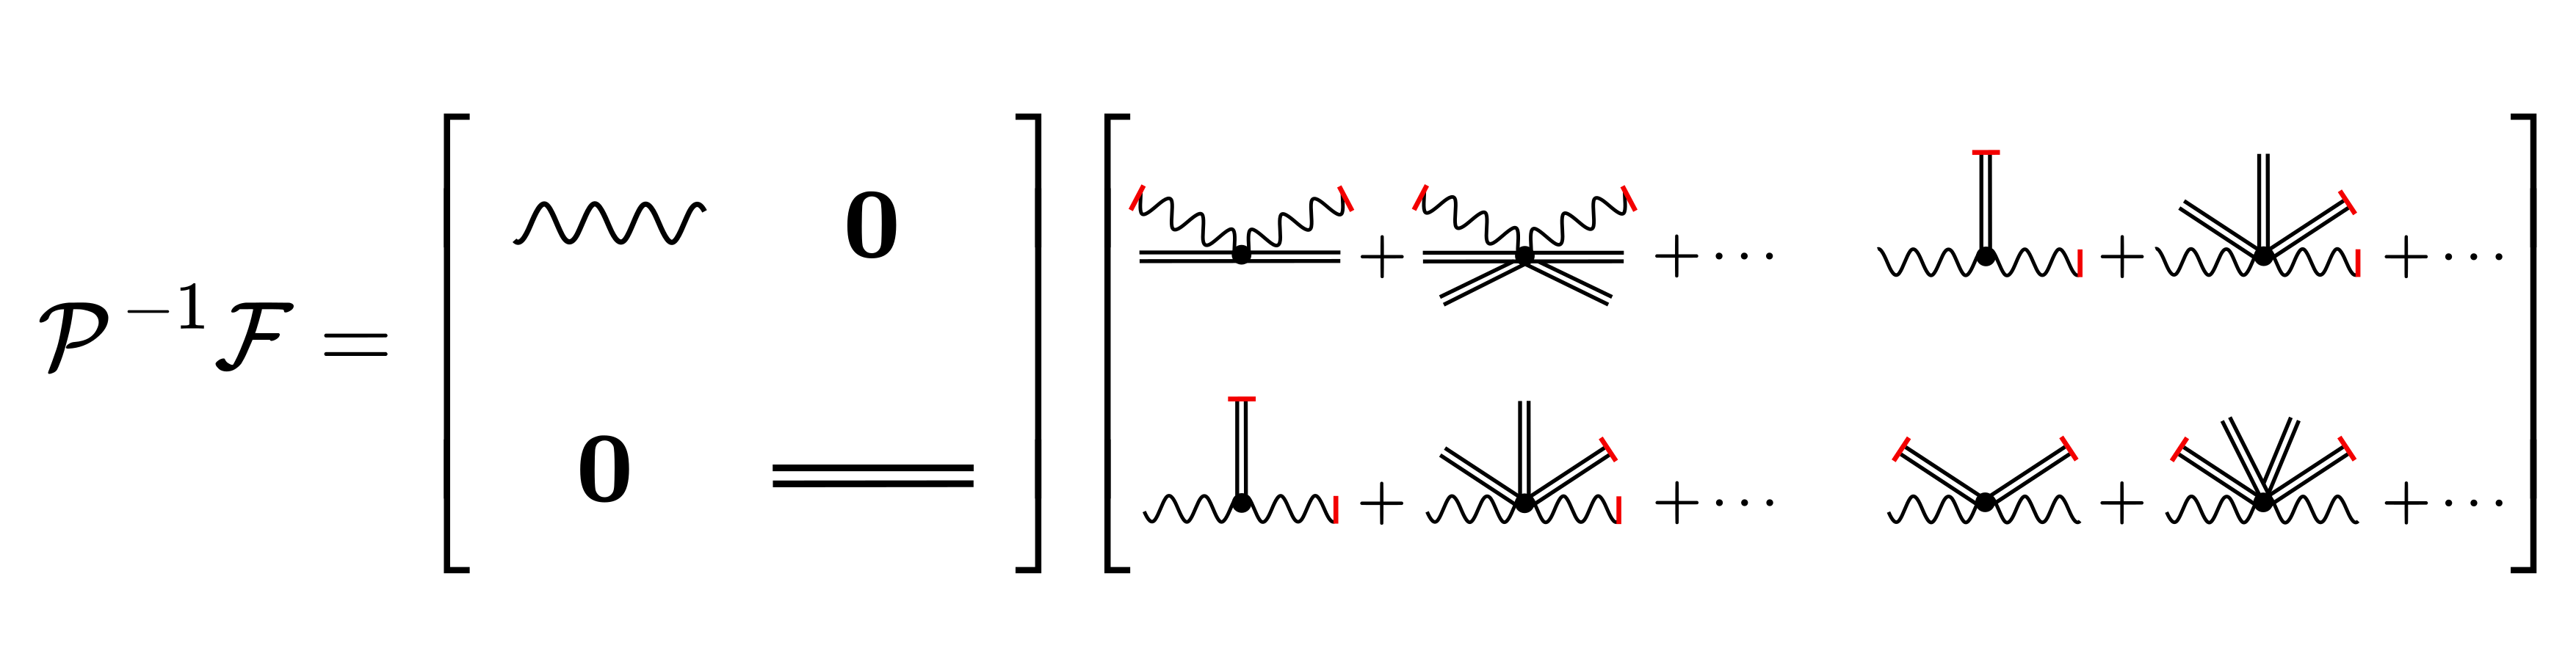
\includegraphics[width=1\textwidth]{./figures/drawing.png}
    \caption*{}
\end{figure}
Where a red line at the end of a vertex leg denotes the functional derivative with respect to the corresponding field.
To extract the gauge field anomalous dimension from the FRGE, we act on it with
a projection operator $\varPi_A$, which then annihilate all terms not originating from diagrams with two external photon legs and leave only the contribution to photon two-point function.
As can be seen, the only vertices that may form such diagrams come from terms of the form $\delta_{A}\delta_h \int c \cdot AAh$ and $\delta_h \delta_h \int c \cdot AAhh$
\begin{figure}[H]
    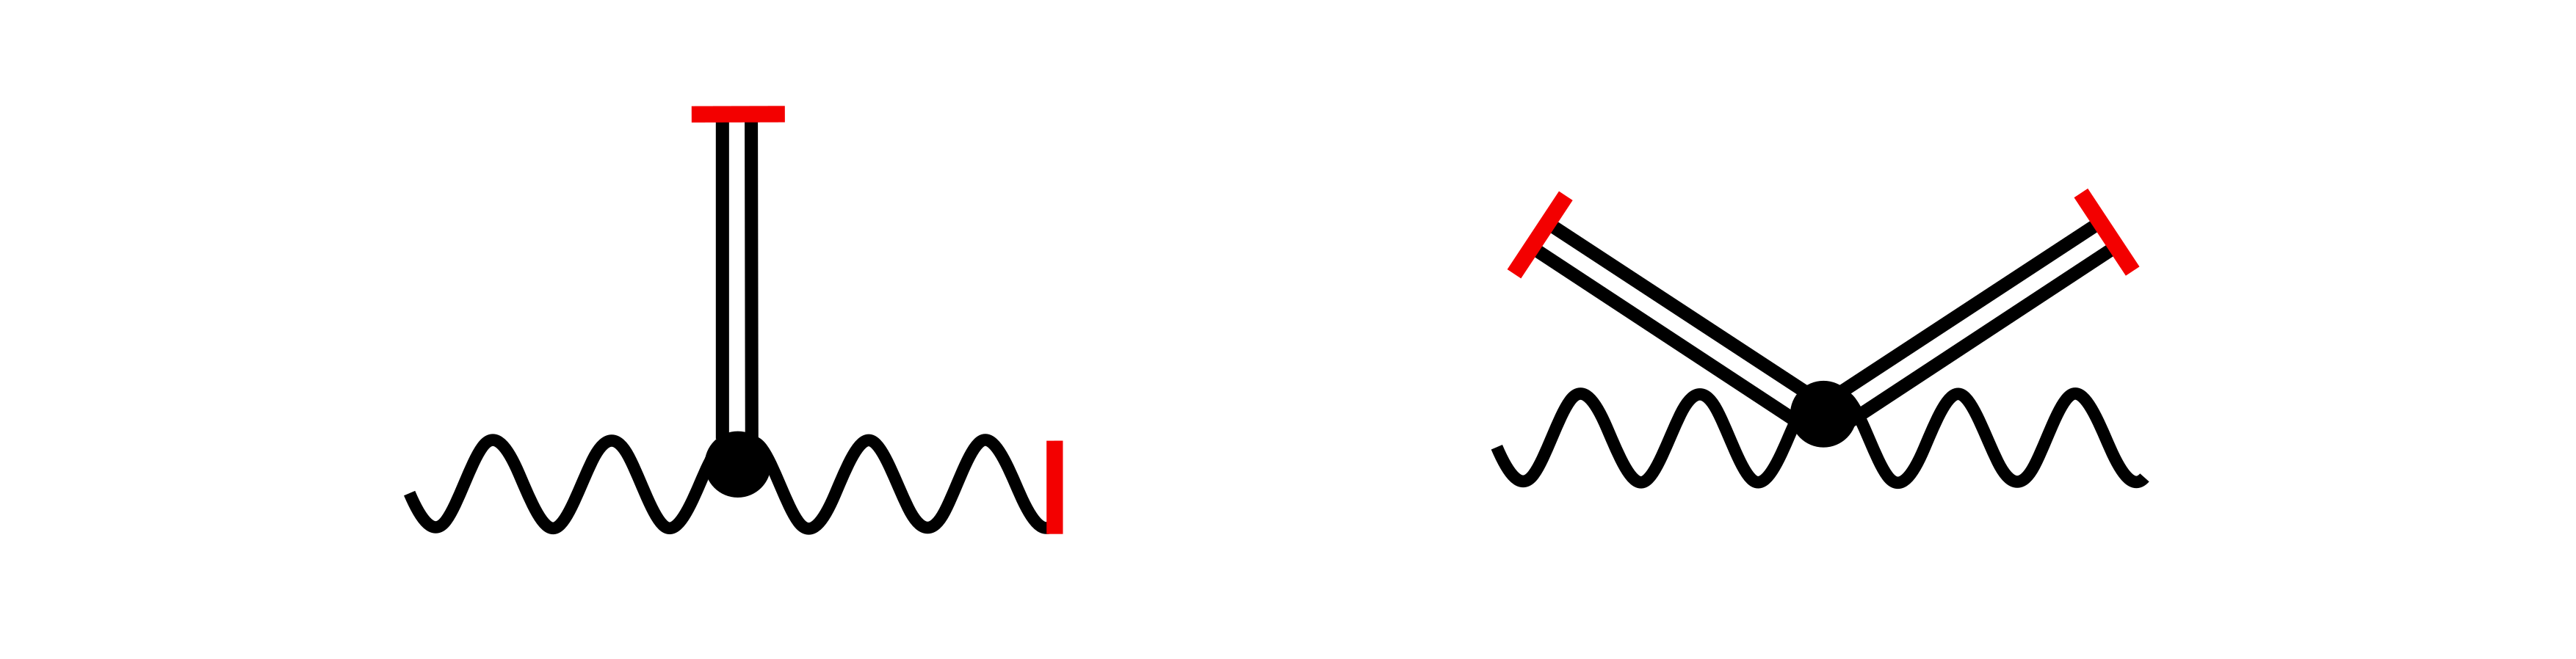
\includegraphics[width=1\textwidth]{./figures/vertices.png}
    \caption{Necessary vertices for computing gauge field anomalous dimension. Red line at the end of a vertex leg denotes a functional derivative with respect to the corresponding field applied to the interaction term}
\end{figure}
We denote the expressions for these vertices, respectively
\begin{gather}
    \left. \frac{\delta^2 \Gamma}{\delta h^{\mu\nu}(p_1) \delta A^{\rho}(p_2)}\right|_{h=0} = \frac{\delta^2}{\delta \tilde{h}^{\mu\nu}(p_1) \delta \tilde{A}^{\rho}(p_2)} \int \prod_{i=1}^3 d^4 p_i \mathcal{L}_{\text{AAh}}\left(\tilde{h}(p_1), \tilde{A}(p_2), \tilde{A}(p_3)\right)\\
    = \operatorname{VertAAh}_{\mu\nu\rho}(p_1,p_2,p_3)\\
    \left. \frac{\delta^2 \Gamma}{\delta h^{\mu\nu}(p_1) \delta h^{\rho\sigma}(p_2)}\right|_{h=0} = \frac{\delta^2}{\delta \tilde{h}^{\mu\nu}(p_1) \delta \tilde{h}^{\rho\sigma}(p_2)} \int \prod_{i=1}^4 d^4 p_i \mathcal{L}_{\text{AAhh}}\left(\tilde{h}(p_1), \tilde{h}(p_2), \tilde{A}(p_3), \tilde{A}(p_4) \right)\\
     = \operatorname{VertAAhh}_{\mu\nu\rho\sigma}(p_1,p_2,p_3,p_4)
\end{gather}
Where $\mathcal{L}_{\text{AAh}}$, $\mathcal{L}_{\text{AAhh}}$ is the sum of terms from lagrangian proportional to the suitable powers of fields.
Full expressions for (..) are given in the appendix.

% A second functional derivative in the FRGE implies, that it has a one-loop structure.

% Our effective action, expanded to second order in metric perturbation field will 

% As we've argued in the previous section, parts of the $\mathcal{F}$ matrix independent of gauge field $A^\mu$ will
% not be projected onto its anomalous dimension. 

%% Opisać "reguły feynmana" i że w tym języku interesować nas będą tylko 1PI poprawki do propagatora fotonu

% In their power series expansion, only quadratic terms will be relevant to the propagator, the rest being responsible for the interaction.
% Przy długich wyrażeniach odsyłać do appendixu

\subsubsection{Calculation of feynman diagrams}
... Then, continuing the argument from previous section, the contribution from second term that will not be annihilated
by $\varPi_A$ comes from products of effective vertices and propagators that involve only the second power of gauge field.
There are just two such products. After considering coefficients in the expansion of logarithm from (\ref{pf}) and from performing trace, the expression for gauge field renormalization beta function can be written as
\begin{align}
    \beta_{Z_A} & = \varPi_A \cdot \partial_t \Gamma_k = \frac{1}{2} \widetilde{\partial_t} \int d^4 q \ \operatorname{VertAAhh}_{\mu\nu\rho\sigma}(p,-p,q,-q) \operatorname{PropG}^{\mu\nu\rho\sigma}(q)\\
    & - \frac{1}{2} \widetilde{\partial_t} \int d^4 q \ \operatorname{VertAAh}^{\mu\nu\rho}(p,-q,p+q) \operatorname{VertAAh}^{\sigma\tau\kappa}(-p,q,-p-q)  \operatorname{PropG}_{\mu\nu\sigma\tau}(p+q) \operatorname{PropA}_{\rho\kappa}(q)
\end{align}
This reduces the problem of extracting information about RG flow in functional renormalization group to computing amputated one-loop feynman diagrams.
\begin{figure}[H]
    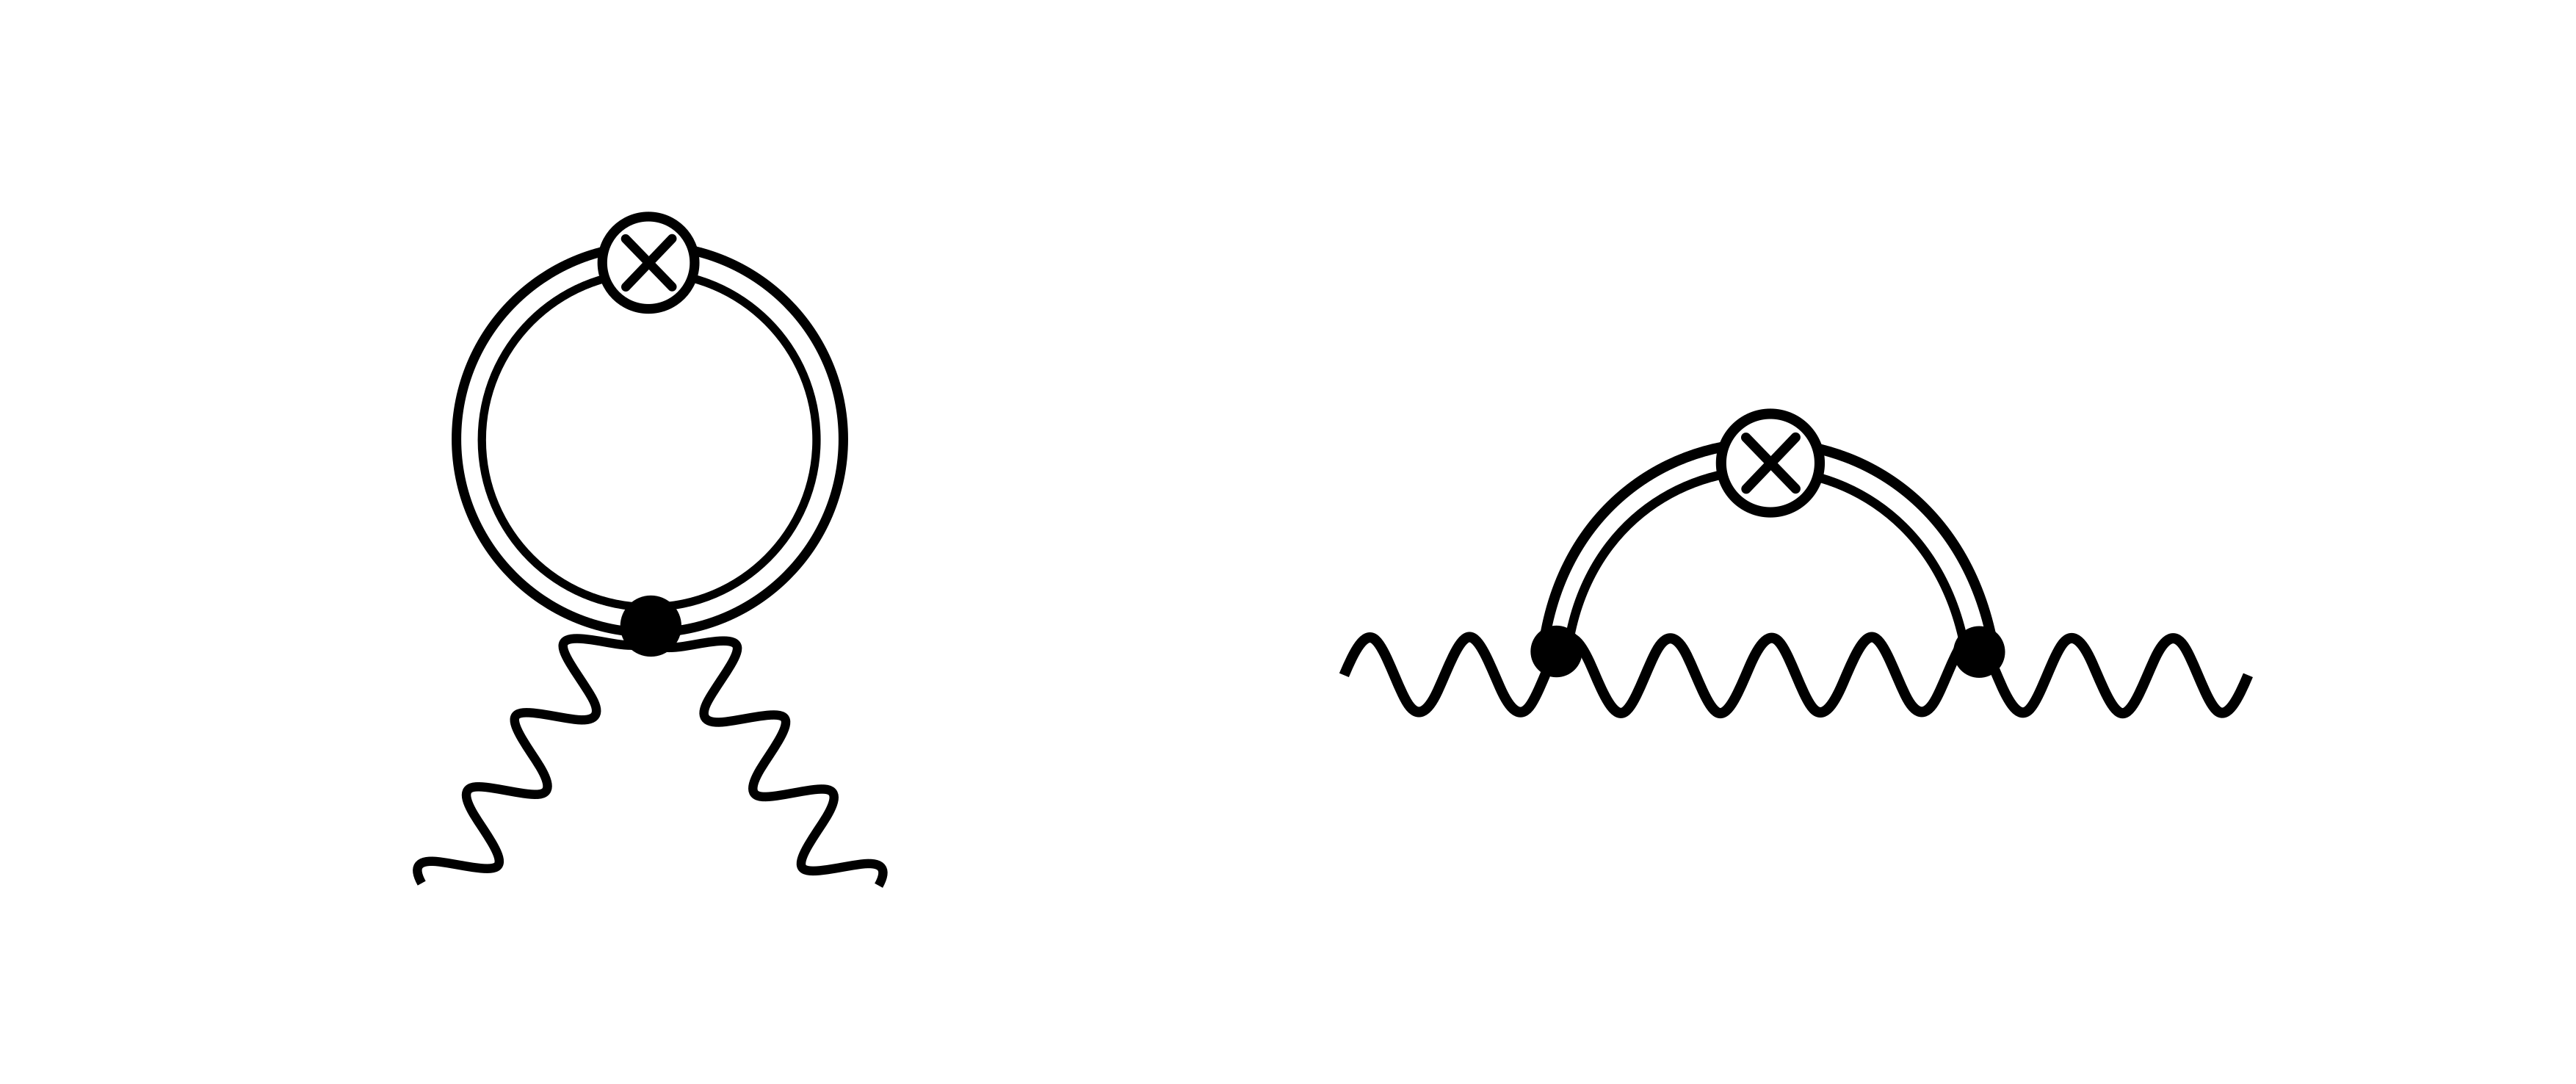
\includegraphics[width=1\textwidth]{./figures/diags.png}
    \caption{Feynman diagrams contributing to the anomalous dimension of gauge field. Wavy line denotes a photon propagator
    and the double straight line denotes the graviton propagator. A crossed circle denotes an insertion of the regulator.}
    \label{diags}
\end{figure} 

% Using the $\mathcal{PF}$-expansion, right hand side of the equation can be represented as the sum of the
% one loop diagrams. 
% %% Projectors
% We are interested in ones contributing to anomalous dimension of gauge field

% Method is as follows. From the effective average action we calculate effective vertices and regulated two-point functions.
% Through the analysis of their allowed tensor structures, we calculate inverses of two-point functions, i.e. propagators.
% Expressions for the 
\textcolor{red}{(...)}\\

Finally, the resulting beta function of abelian gauge coupling $g$ in the spacetime with four dimensions is
\begin{equation}
    \beta_{g_Y} = g_Y \frac{\eta_A}{2} = g_Y \frac{G}{4 \pi} \left( \frac{\eta_h - 6}{6(1-2 \Lambda)^2} - 
    \frac{(\eta_A-8)(1-2\Lambda) + (\eta_h -8)}{8 (1-2 \Lambda )^2}\right) + \beta_{g_Y}^{\text{SM}}
\end{equation}
Beta function for an arbitrary spacetime dimensionality is given in (apx).



Beta functions extracted from the full EA cannot depend on the choice of gauge parameters.
Introducing truncations, however, means that gauge dependence may not cancel entirely (...).
%% ?? Że będziemy sprawdzać zależność od gauge parameter ?? - tylko od beta w gravity gauge fixing (z jakiegoś powodu) - na alfy możemy też zrobić rg flow i one jakoś dążą do zera i jest argument że są nieważne (poczytać)
Another in principle redundant choice is a form of the regulator. For two different regulators,
$\Gamma_k$ will include field modes weighted in a different manner, so this choice simply
sets the definition of the object $\Gamma_k$. 
This means, that beta functions computed with different regulators will differ, but
if the regulator is picked in such way that it executes a proper IR cutoff,
it will always give the same results in the physical limit $k \rightarrow 0$. There should be no
qualitative differences in the behaviour of RG flow computed with different regulators.
%% Coś o tym że to będziemy tu sprawdzać


%%% CO JEST JESZCZE DO UWZGLĘDNIENIA %%%
%% Systematycznie wypisać wszystkie wykorzystywane przybliżenia i przedyskutować ich wpływ, ważność i możliwą weryfikację czy działają
%% Wick rotation
%% Fourier transforms of lagrangian and 
%% O LINEAR SPLIT I ŻE WOKÓŁ FLAT BACKGROUND
%% Why we skip ghosts



\section*{Summary}

\begin{thebibliography}{9}
    \bibitem{betaf scalar}
    Brod, J., Polonsky, Z. Two-loop beta function for complex scalar electroweak multiplets. J. High Energ. Phys. 2020, 158 (2020). https://doi.org/10.1007/JHEP09(2020)158
    \bibitem{betaf chiral lagrangian}
    Buchalla, G., Catà, O., Celis, A., Knecht, M., Krause, C., Complete one-loop renormalization of the Higgs-electroweak chiral Lagrangian. Nuclear Phys. B 2018, 928 (93). https://doi.org/10.1016/j.nuclphysb.2018.01.009
\end{thebibliography}

\end{document}